% D7 草稿存档（2026-10-25）: 应用户要求从 overleaf/sections/sec6_results.tex 撤回, overleaf 已恢复为原模板。
% 待用户核验图表与文字后, 在 D8 阶段最后写回 overleaf。恢复方法:
%   cp "docs/D7_sec6_results_draft_v1.0.tex" overleaf/sections/sec6_results.tex (去掉本 3 行注释头)
% 源提交: 053de96(D7初稿)+af8d4e3(Holm勘误)+0032717(PULL提醒, 随撤回作废)

\section{Results and Evaluation}
\label{sec:results}
% D owns this file: metrics, figures, cross-dataset comparison, and statistical analysis.
%
% *** E: PULL FROM GITHUB FIRST (2026-10-25) before editing this file or sec7. ***
% D delivered the full sec6 draft + figures (fig_d_*.pdf in overleaf/figures/) + the
% 3-sentence verified summary (comment block at top of sec7). If you started writing
% these sections on Overleaf without pushing, reconcile before pushing to avoid
% overwriting. Compilation checklist and your TODOs: docs/D7_结果章初稿_v1.0.md §4.
%
% All numbers trace to results/all_metrics_v1.csv (D4), results/cross_dataset_comparison_v1.csv
% (D6), and results/ttest/ (C5/C11). Figure sources: figures/fig_d_sources.csv.

\subsection{Evaluation Setup and Reporting Conventions}
\label{sec:results-setup}

All 32 main-matrix configurations (four classifiers $\times$ four imbalance strategies $\times$ two datasets) were evaluated under the two locked protocols: stratified 10-fold cross-validation (cv10, seed 42) and a stratified 70:30 holdout evaluated once after all settings were fixed. Every reported number derives from the archived fold-level and pooled out-of-fold predictions; means are over the 10 folds with population standard deviation (ddof $=0$), and confusion matrices are pooled over folds. The positive class is \texttt{bad} for credit-g and \texttt{sick} for sick. F1, precision, and recall refer to the positive class throughout; AUC is computed from out-of-fold positive-class probabilities. Threshold-adjusted models selected their threshold $\tau$ on development folds only (observed range 0.20--0.60); their AUC is bitwise identical to the plain model's, confirming that $\tau$ moves the operating point and not the score ranking. A ZeroR baseline (majority class) is included as a reference, not as a competitor: it reaches 70.0\% accuracy on credit-g and 93.9\% on sick with zero recall, which is exactly the accuracy--recall trap this project studies.

\subsection{credit-g: Accuracy Is Cheap, Minority Recall Is Not}
\label{sec:results-creditg}

\begin{table}[H]
\centering
\caption{credit-g, cv10 F1 (mean $\pm$ std over 10 folds; positive class \texttt{bad}). Champion in \textbf{bold}. Full metric set: \texttt{results/all\_metrics\_v1.csv}.}
\label{tab:creditg-f1}
\begin{tabular}{lcccc}
\toprule
Model & Plain & SMOTE & Cost-sensitive & Threshold \\
\midrule
Decision Tree & $0.322\pm0.192$ & $0.471\pm0.078$ & $0.523\pm0.030$ & $0.561\pm0.038$ \\
Random Forest & $0.499\pm0.079$ & $0.509\pm0.077$ & $0.595\pm0.064$ & $0.595\pm0.059$ \\
Logistic Reg. & $0.531\pm0.060$ & $0.591\pm0.051$ & $\mathbf{0.597\pm0.034}$ & $0.591\pm0.049$ \\
SVC & $0.498\pm0.101$ & $0.560\pm0.050$ & $0.593\pm0.032$ & $0.590\pm0.055$ \\
\midrule
ZeroR (ref.) & \multicolumn{4}{c}{F1 $=0$ (acc.\ 0.700, recall 0)} \\
\bottomrule
\end{tabular}
\end{table}

Table~\ref{tab:creditg-f1} shows the cv10 F1 landscape. Three observations:

\textbf{(i) Plain models fall into the accuracy trap.} The three plain tree/kernel models (DT, RF, SVC) sit at or below ZeroR-level recall (0.27--0.40), trading minority detection for majority-class accuracy (0.71--0.77); their plain F1 (0.32--0.50) is the worst column. This is the RQ2 pattern: high accuracy is achievable while detecting almost no bad credit.

\textbf{(ii) Every intervention helps here.} All three strategies lift F1 for every model on credit-g (mean $\Delta$F1 $+0.070$ to $+0.122$); the champion is \emph{cost-sensitive logistic regression} (\texttt{lr\_cost}, F1 $0.597\pm0.034$, recall $0.863$ vs.\ $0.470$ plain, precision $0.457$), which moves the decision boundary without synthesising data or adding capacity. Its pooled confusion cost $(5\,\mathrm{FN}+\mathrm{FP})/N$ drops to $0.514$ from $0.884$ (plain LR).

\textbf{(iii) The holdout agrees.} On the 70:30 holdout, \texttt{lr\_cost} reaches F1 $0.580$ / recall $0.822$, within one standard deviation of the cv10 estimate --- no setting was tuned on the holdout.

\subsection{sick: Strategies Move the Operating Point, Not the Ranking}
\label{sec:results-sick}

\begin{table}[H]
\centering
\caption{sick, cv10 F1 (mean $\pm$ std; positive class \texttt{sick}). Champion in \textbf{bold}. DT/LR/SVC cost rows equal plain because cost weighting changed no prediction (bitwise-identical pooled confusion matrices).}
\label{tab:sick-f1}
\begin{tabular}{lcccc}
\toprule
Model & Plain & SMOTE & Cost-sensitive & Threshold \\
\midrule
Decision Tree & $0.836\pm0.050$ & $0.747\pm0.051$ & $0.836\pm0.050$ & $0.820\pm0.048$ \\
Random Forest & $0.870\pm0.047$ & $\mathbf{0.897\pm0.051}$ & $0.873\pm0.048$ & $0.877\pm0.052$ \\
Logistic Reg. & $0.687\pm0.091$ & $0.521\pm0.028$ & $0.687\pm0.091$ & $0.745\pm0.038$ \\
SVC & $0.763\pm0.064$ & $0.742\pm0.039$ & $0.763\pm0.064$ & $0.809\pm0.039$ \\
\midrule
ZeroR (ref.) & \multicolumn{4}{c}{F1 $=0$ (acc.\ 0.939, recall 0)} \\
\bottomrule
\end{tabular}
\end{table}

The sick landscape differs structurally from credit-g. First, \textbf{SMOTE hurts the models it should help}: it is the only strategy that reduces F1 for DT ($-0.089$, $p=0.048$) and collapses logistic regression ($-0.166$, $p=0.002$), while leaving Random Forest intact ($+0.027$, n.s.). Second, \textbf{cost weighting is an exact identity map} for DT, LR, and SVC: with only 6.1\% positives, the predicted probabilities are too extreme for the class-weight adjustment to flip any test instance across the 0.5 boundary, so the pooled confusion matrices are bitwise identical to plain (Random Forest is the exception, consistent with its probability calibration). Third, Figure~\ref{fig:rocpr} shows the three strategies' ROC and PR curves nearly coincide (AUC $0.997$--$0.998$ for Random Forest): the interventions move the \emph{operating point}, not the score ranking, so their entire effect is a precision--recall trade along an essentially fixed curve.

\begin{figure}[H]
\centering
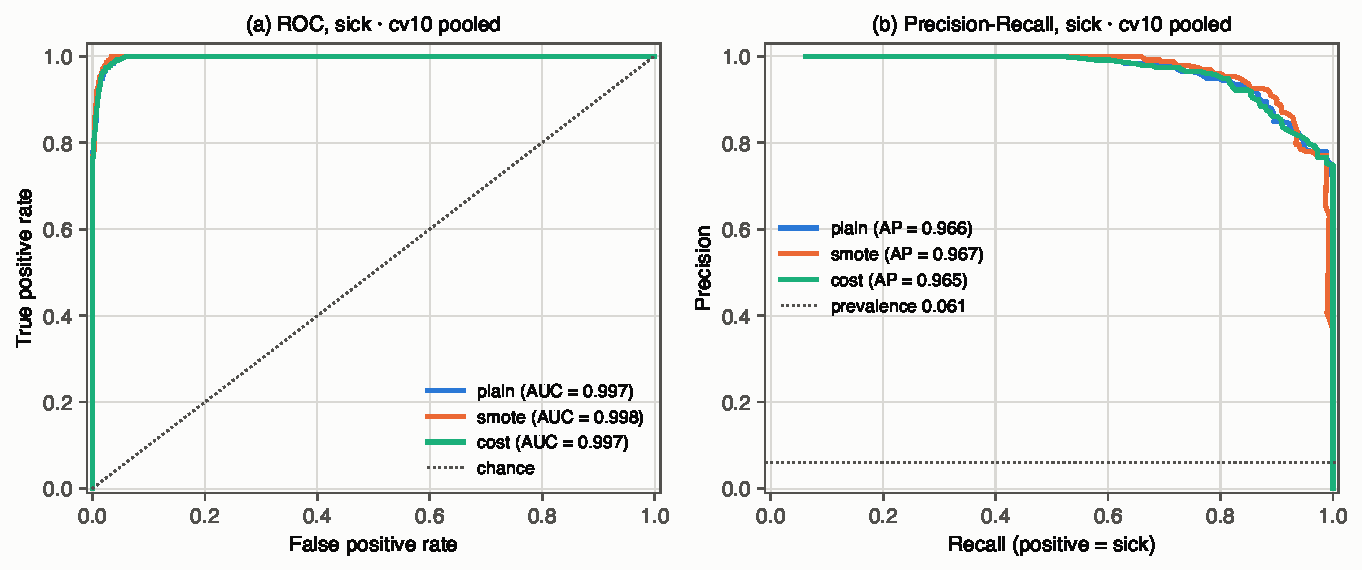
\includegraphics[width=\textwidth]{figures/fig_d_sick_roc_pr.pdf}
\caption{ROC (a) and Precision--Recall (b) curves on sick for Random Forest under plain, SMOTE, and cost-sensitive strategies, computed from pooled out-of-fold predictions of the 10-fold cross-validation protocol (all 3{,}772 instances; positive class \texttt{sick}). Dotted lines mark chance level (a) and the positive-class prevalence $231/3772=0.061$ (b). The curves nearly coincide: ranking quality is strategy-invariant. Source data: \texttt{results/preds/sick\_rf\_*\_v1\_run1\_cv10\_preds.csv}.}
\label{fig:rocpr}
\end{figure}

\subsection{Strategy Effects and Statistical Significance}
\label{sec:results-sig}

\begin{figure}[H]
\centering
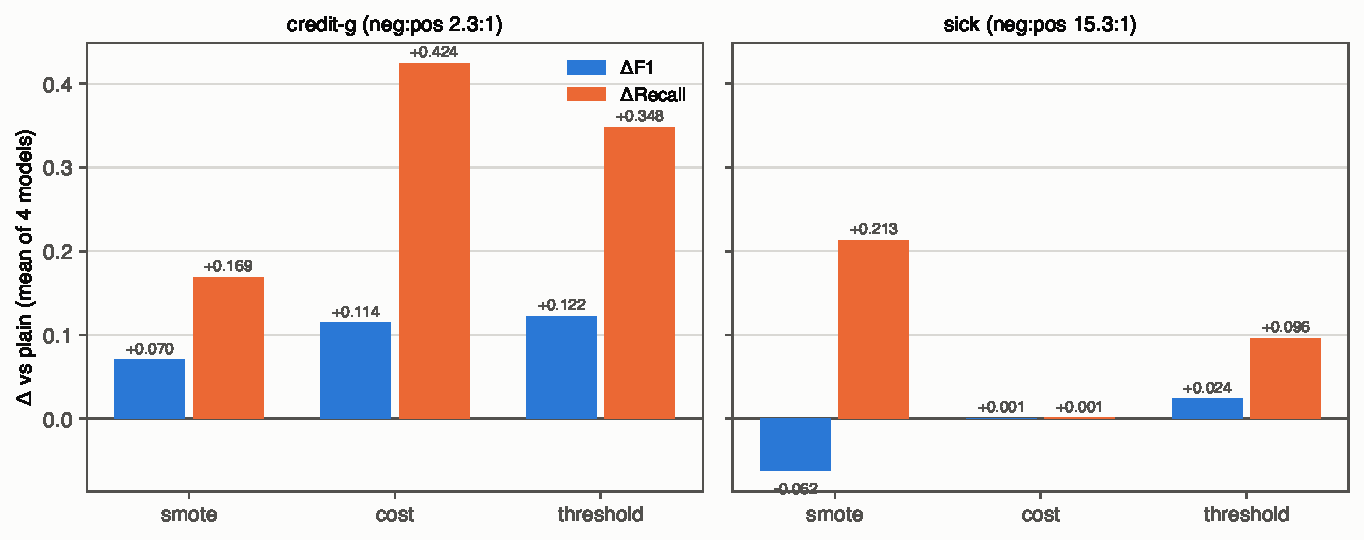
\includegraphics[width=\textwidth]{figures/fig_d_strategy_gain.pdf}
\caption{Effect of each imbalance-handling strategy relative to plain training, averaged over the four base models (cv10): $\Delta$F1 (blue) and $\Delta$Recall (orange), $\Delta=$ strategy $-$ plain, from the twelve pre-specified paired comparisons per metric (Nadeau--Bengio corrected $t$-tests). Left: credit-g (positive \texttt{bad}, 30.0\%, neg:pos 2.3:1); right: sick (positive \texttt{sick}, 6.1\%, neg:pos 15.3:1). Recall gains are non-negative everywhere while F1 gains flip sign on sick. Source: \texttt{results/cross\_dataset\_comparison\_v1.csv}.}
\label{fig:gain}
\end{figure}

Twelve pre-specified strategy-vs-plain comparisons per metric were tested with fold-level paired $t$-tests corrected for fold overlap following Nadeau and Bengio (variance factor $1/k + n_2/n_1 = 0.2111$, i.e.\ 2.11$\times$ the naive variance --- deliberately conservative). Stars in the text denote raw $p$ at $\alpha=0.05$ ($^{*}<0.05$, $^{**}<0.01$, $^{***}<0.001$); we additionally state the Holm (1979) outcome within each full family of 120 pairs, and it splits by metric. In the F1 families none of the twelve pre-specified contrasts survives Holm, and on credit-g only one pair of all 120 does (\texttt{dt\_smote} vs \texttt{lr\_smote}, $p_{\mathrm{Holm}}=0.021$); on sick 22 pairs survive, almost all of the form ``every configuration beats the collapsed \texttt{lr\_smote}/\texttt{svc\_smote}''. The credit-g recall gains, by contrast, are Holm-robust: 8 of the 12 pre-specified recall contrasts survive (all cost/threshold). We therefore report the pre-specified contrasts at raw $p$ and state the Holm outcome per metric rather than hide it. Figure~\ref{fig:gain} summarises the pattern:

\begin{itemize}
  \item \textbf{Recall gains are same-direction everywhere}: all twelve comparisons raise recall (credit-g $+0.06$ to $+0.59$, sick $+0.004$ to $+0.28$), nine significantly.
  \item \textbf{F1 gains flip across datasets}: three sign flips on sick (DT and LR $\times$ SMOTE, DT $\times$ threshold), all concentrated in SMOTE$\times$(DT/LR). The strategies reliably buy recall; the precision price is what depends on the dataset.
  \item \textbf{Accuracy drops almost everywhere} (credit-g cost/threshold $-0.04$ to $-0.19$, mostly significant; sick $\leq 0.07$): minority gains are paid for in majority-class accuracy, and accuracy alone would have hidden them.
\end{itemize}

\subsection{Cross-Dataset Comparison: The Winner Flips}
\label{sec:results-flip}

\begin{figure}[H]
\centering
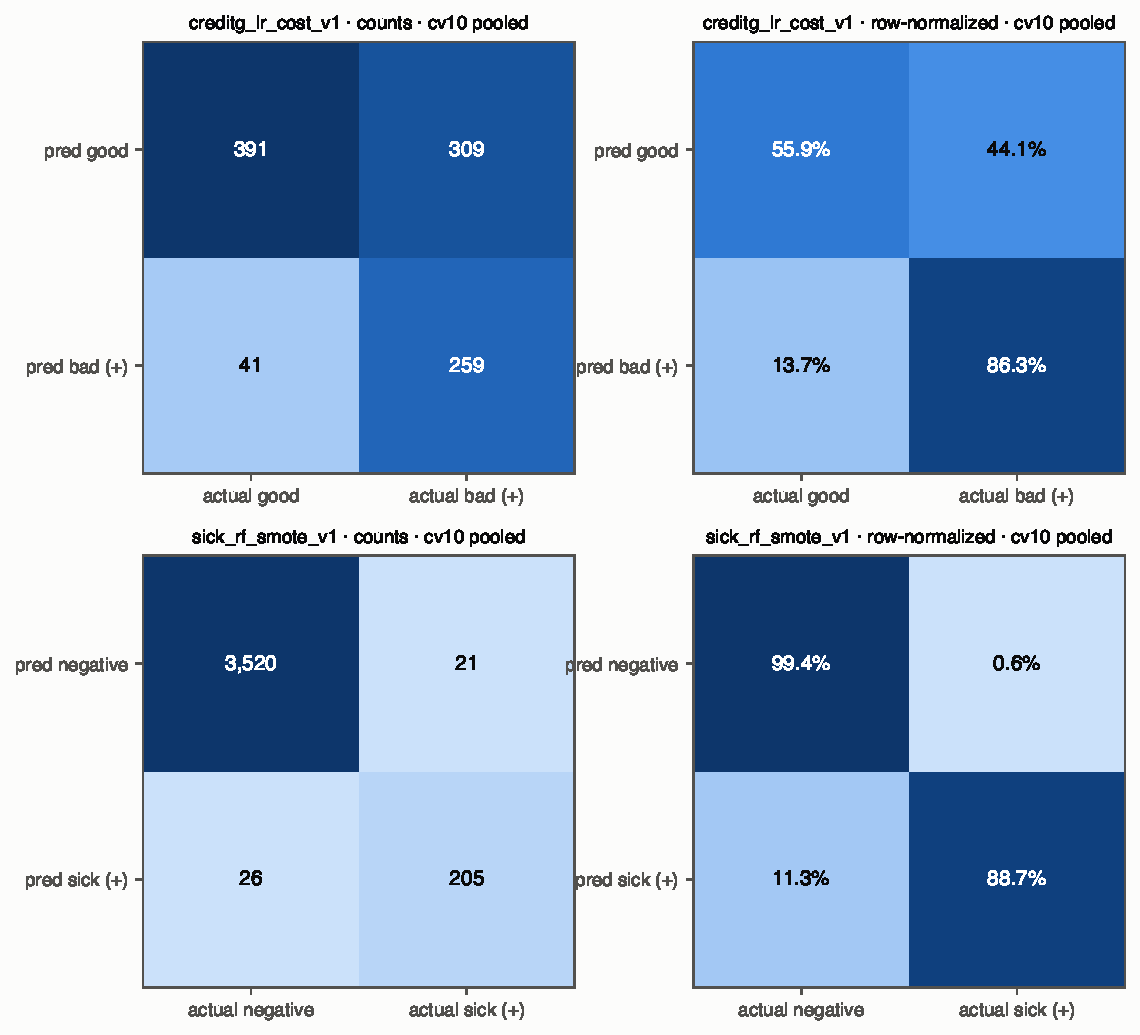
\includegraphics[width=0.8\textwidth]{figures/fig_d_confusion.pdf}
\caption{Confusion matrices of the per-dataset F1 champions (cv10, pooled out-of-fold predictions; rows = predicted, columns = actual; $(+)$ marks the positive class): credit-g \texttt{lr\_cost} (top, positive \texttt{bad}) and sick \texttt{rf\_smote} (bottom, positive \texttt{sick}). Left: counts; right: row-normalised. Source: \texttt{results/all\_metrics\_v1.csv}.}
\label{fig:confusion}
\end{figure}

The two datasets crown different winners (Figure~\ref{fig:confusion}): credit-g rewards \emph{linear + cost-sensitive} (\texttt{lr\_cost}, F1 $0.597$, recall $0.863$, precision $0.457$ --- it catches 259 of 300 bad cases but flags 309 of 700 good ones), while sick rewards \emph{ensemble + resampling} (\texttt{rf\_smote}, F1 $0.897$, recall $0.888$, precision $0.910$ --- near-clean on both error types). A naive single-variable reading --- ``more imbalance needs more resampling'' --- predicts SMOTE should help \emph{more} on sick (15.3:1) than credit-g (2.3:1); the data say the opposite. Four dataset properties jointly explain the flip:

\textbf{Size (1{,}000 vs 3{,}772 rows).} On credit-g, high-capacity learners (RF, AdaBoost, $n_{\mathrm{estimators}}=100$) train on only 900 rows per fold and their variance dominates; a strong-prior linear model plus an intervention that only re-weights the loss (cost) is the stable choice. On sick, capacity pays: bagging reduces variance and boosting reduces bias on 3{,}395-row training folds.

\textbf{Attribute composition (13 vs 22 categorical attributes).} SMOTE interpolates linearly in the one-hot-encoded space, synthesising fractional categories (``half-open door''); sick's sparser one-hot space amplifies this interpolation noise. The linear decision surface of LR is most sensitive (F1 $-0.166$, $p=0.002^{**}$), whereas axis-parallel tree splits depend only on feature ordering and are insensitive (RF $+0.027$, n.s.).

\textbf{Missingness (0\% vs 29.9\% of rows).} sick's imputation noise further penalises distance- and hyperplane-based learners (LR, SVC), while tree ensembles are rank-robust to it --- widening the tree-vs-linear gap that the champion comparison shows.

\textbf{Imbalance (2.3:1 vs 15.3:1).} Imbalance explains \emph{strategy choice}, not model choice: at 30\% positives, class weighting suffices to move many boundary cases (recall $+0.34$ to $+0.59^{***}$); at 6.1\% positives, DT/LR/SVC probabilities are too polarised for the weight change to flip any prediction (the identity map of Section~\ref{sec:results-sick}), and recall must instead be bought by explicit synthesis (SMOTE) or iterative re-weighting (boosting).

In short: small, complete, moderately imbalanced credit-g rewards \emph{correct priors + cost sensitivity}; large, noisy, extremely imbalanced sick rewards \emph{capacity + resampling}. No single dimension predicts the winner.

\subsection{Ensemble Study (Exploratory)}
\label{sec:results-ensemble}

As an exploratory extension outside the pre-registered main matrix, bagging (BaggingClassifier) and AdaBoost were run $\times$ \{plain, SMOTE\} $\times$ both datasets under the same locked cv10 protocol. The ensemble results are reported as an exploratory extension; only two pre-specified comparisons were tested, and the remaining cells are descriptive mean $\pm$ std only.

\begin{table}[H]
\centering
\caption{Ensemble study (exploratory), cv10 (mean $\pm$ std over 10 folds). F1 for the positive class; best exploratory F1 per dataset in \textbf{bold}. Ensemble models are not part of the main matrix or its statistical family. Source: \texttt{results/ensemble\_metrics\_v1.csv}.}
\label{tab:ensemble}
\begin{tabular}{llcccc}
\toprule
Dataset & Config & F1 & Recall & AUC & Runtime (s) \\
\midrule
credit-g & bag+plain & $0.510\pm0.072$ & 0.430 & 0.782 & 2.2 \\
credit-g & bag+SMOTE & $0.548\pm0.074$ & 0.560 & 0.771 & 1.2 \\
credit-g & ada+plain & $0.500\pm0.070$ & 0.473 & 0.735 & 1.2 \\
credit-g & ada+SMOTE & $0.501\pm0.087$ & 0.483 & 0.723 & 2.4 \\
\midrule
sick & bag+plain & $0.819\pm0.050$ & 0.775 & 0.990 & 3.6 \\
sick & bag+SMOTE & $0.785\pm0.037$ & 0.987 & 0.994 & 4.6 \\
sick & ada+plain & $0.918\pm0.046$ & 0.901 & 0.999 & 9.5 \\
sick & ada+SMOTE & $\mathbf{0.937\pm0.044}$ & 0.931 & 0.999 & 28.9 \\
\bottomrule
\end{tabular}
\end{table}

The two pre-specified tests (Nadeau--Bengio corrected, as above) were \texttt{bag\_plain} vs \texttt{dt\_plain} (does bagging reduce the single-tree's variance?) and \texttt{ada\_plain} vs \texttt{dt\_smote} (does boosting's re-weighting substitute for resampling?):

\begin{itemize}
  \item \texttt{bag\_plain} vs \texttt{dt\_plain}: credit-g $+0.188$, $p=0.071$ (n.s.); sick $-0.018$, $p=0.067$ (n.s.).
  \item \texttt{ada\_plain} vs \texttt{dt\_smote}: credit-g $+0.028$, $p=0.389$ (n.s.); \textbf{sick $+0.171$, $p=6.4\times10^{-4***}$}.
\end{itemize}

The one significant result: on sick, boosting's iterative re-weighting significantly outperforms SMOTE resampling at the same base learner --- consistent with \texttt{ada\_smote} posting the highest sick F1 of the whole project ($0.937$). We note that \texttt{ada\_smote} ($0.937$) vs main-matrix champion \texttt{rf\_smote} ($0.897$) was \emph{not} a tested comparison and is descriptive only.

Two zero-cost insights follow from reading Table~\ref{tab:ensemble} against the main matrix, with no additional experiments:

\textbf{(1) Why tree ensembles absorb SMOTE.} \texttt{bag+SMOTE} on sick pushes recall to $0.987$ but F1 \emph{drops} to $0.785$ (precision collapses), while \texttt{ada+SMOTE} converts the same resampled data into balanced gains ($0.931$ recall, $0.943$ implied precision). Combined with the main-matrix finding that SMOTE leaves RF intact but hurts LR, this supports the axis-parallel-split explanation: tree ensembles are robust to one-hot interpolation noise, and boosting additionally re-weights the noisy synthetic minority examples down over rounds instead of trusting them equally.

\textbf{(2) Why the bag/ada ranking flips with the dataset.} On credit-g both ensembles trail the main champion (\texttt{lr\_cost} $0.597$) --- with 900-row training folds, added capacity overfits; on sick both lead every single model --- with 3{,}395-row folds, capacity compounds with resampling. The ensemble flip mirrors the main-matrix winner flip and reinforces the size/attribution story of Section~\ref{sec:results-flip}.
